\documentclass[../main.tex]{subfiles}
\usepackage{graphicx}

\begin{document}
\textbf{Component 3: Individual Questions (Data Science)}
\newline 
What technical or professional skills have you identified as relevant to the project?
\newline
\newline
\textbf{Learning: Level 5 ( MLNG )}
Machine learning [2] as genetic algorithms can be used to approximate a model through trial and error. This was a skill I thought was quite important because it's almost completely automated and you can save a significant amount of time through implementing methods such as simulated annealing, crossover etc. The method I thought to be the most useful was simulated annealing as it starts at a high temperature and reduces the temperature until eventually approximates to a global minimum. This allowed me to reach a near optimal model in little time.
\newline
\newline
 I applied this skill in python with the library \textbf{PyGAD} [1] to implement these algorithms to help with approximating a model. \newline
\newline
\textbf{Database design SFIA 9 Level 5 (DBDS):}
The initial problem with big data will always be sifting through and structuring large amounts of data in a manner that is cohesive and easily accessible. This is why database design [6] was a highly important skill for this task. In the context of forecasting natural disasters, many types of data are required to forecast depending on the type of natural disaster, which is why taking the time to plan out and structure data with a clear goal in mind, significantly improves the efficiency and analysis that can be made with the data and reduces the likelihood of premature conclusions made on data later along the process.
\newline
\newline
To apply this skill I first planned out how I wanted to organise my data. Then I used \textbf{SQL} to clean and structure my data I also used google cloud bigquery [4] to run my sql.
\newline
\newline
\textbf{Data visualisation SFIA 9 Level 5 (DTAN):}
Picking a model that accurately represents your data is crucial to analysing trends and general relationships. This is because a good model significantly helps to engage and communicate ideas to stakeholders [5] and display general trends to help provide justification for prediction through the extrapolation of data. Spending the time selecting a good model is important as a regression model might accurately represent the data pool but past the set of values within your data pool, making it useless for making predictions. 
\newline
\newline
To apply this skill I used the language R and the IDE R studio and used regression models to see general trends and modeled data as well as format my data in a clear and concise manner.
\newline
\newline
\textbf{How did you approach the problem as a team, and what challenges did you encounter in working together?}
\newline
\newline
Approaching the problem as a team allowed us to listen to each other's ideas and tackle challenges head on. During our meetings we allocated time to help each other with their ongoing problems to help reason provide our own perspectives on the problem.
\newline
\newline
\textbf{Computer Science:} Was having problems with \textbf{premature convergence} with a \textbf{genetic algorithm} when approximating a model for a set of data. He helped me suggest a \textbf{uniform crossover} to help prevent this [15]. 
\newline
\newline
\textbf{Software development:} listened and provided their input and allowed me to improve the structure of my \textbf{SQL} tables 
\newline
\newline
\textbf{Cyber Security:} Gave insight on certain security measures he thought could be effective to implement with handling my database.
\newline
\newline
\textbf{What professional or technical skills have you identified you need to develop or fine tune}?
\newline
\newline
\textbf{Database design} [6]: I believe this an important skill and my ability to design a database for this scenario was adequate. I personally feel that I could improve on it further and fine tune it more as there were moments where I wasn’t completely confident and had to ask questions to the group as mentioned above. Another reason why I would like to work on it further is I feel like it's an important skill to develop with sql being almost applicable to a large amount of areas in computer science. Furthermore, I believe there is always more to learn regarding designing and implementation of a database.
\newline
\newline
\textbf{Numerical analysis:} I would like to develop my numerical analysis more as it's always been a weak point for me. I think overall it improved during the course of this project as I was able to spend a significant time using machine learning to create an algorithm to approximate a model and I also practiced linearising relationships to display the relationship between 2 variables. Which I feel like is a step in the right direction. But I think I need to work on it further and hone my skills more into this area as it's an important fundamental for understanding deeper and more difficult concepts.
\newline

\textbf{Pulling from git}

 \centering{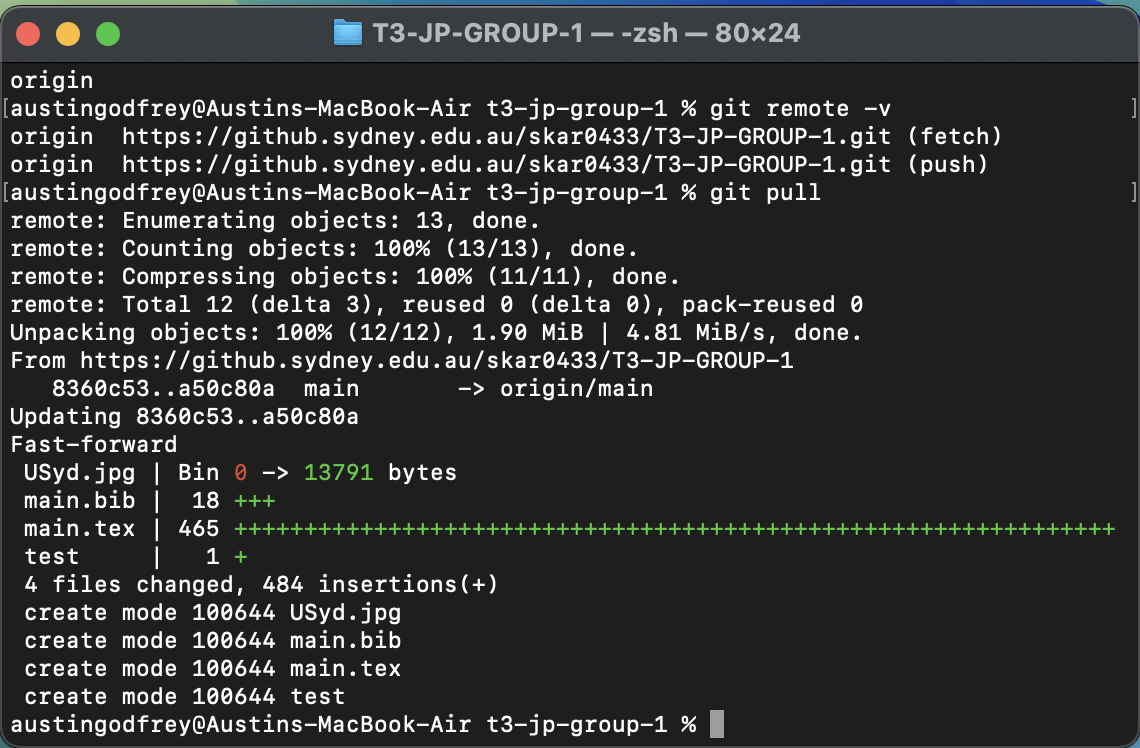
\includegraphics[width=0.8\textwidth]{git_pull}}
 \newline
 - Typed git pull in terminal to pull from the repo
\newline

\textbf{Pushing to git}
\newline

 1) Typed git add followed by the filepath in terminal to stage the file
 \newline
 \centering{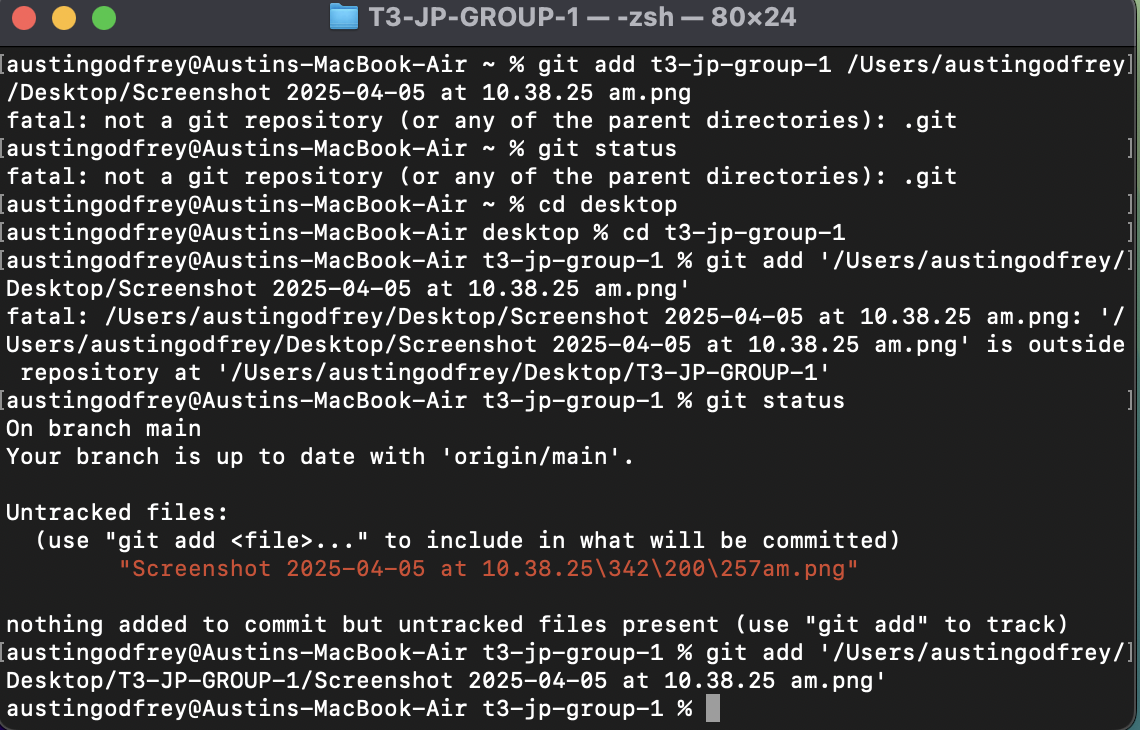
\includegraphics[width=0.8\textwidth]{austinpushfiles/add_to_staging.png}}

 \textbf{2) Used git commmit to commit the file to the main branch}
 \newline
 \centering{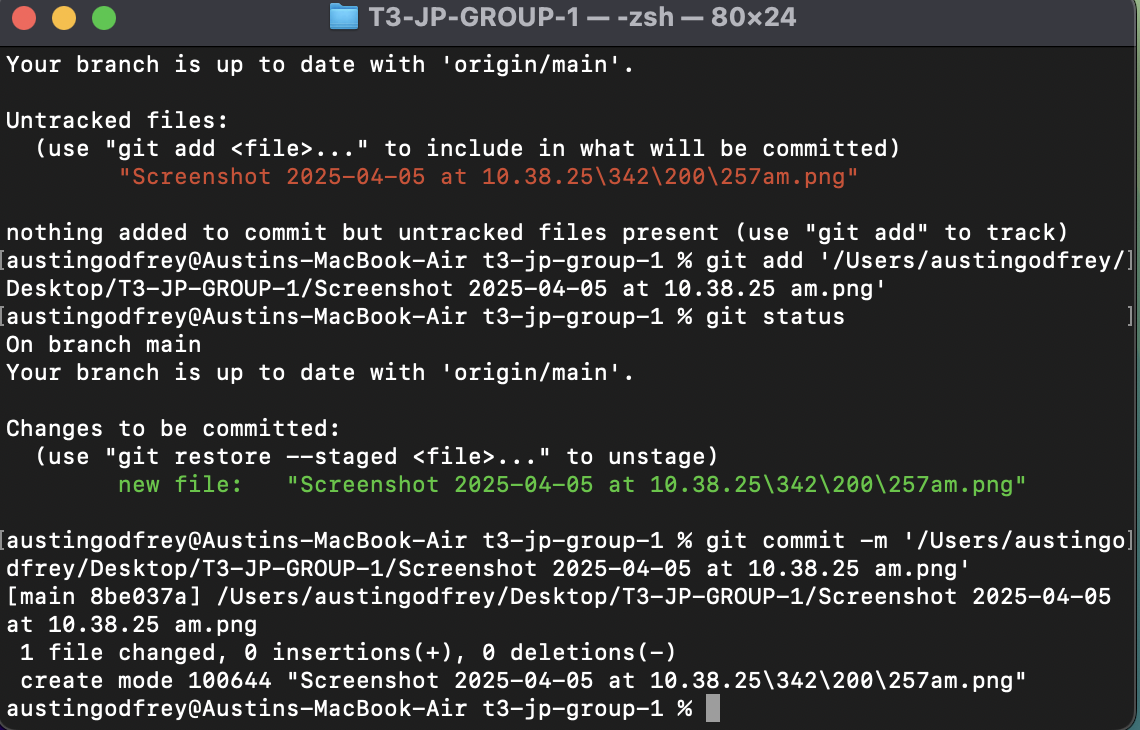
\includegraphics[width=0.8\textwidth]{austinpushfiles/commit_to_main.png}}

 3) Finally use git push to push the changes to the main branch
 \newline
 \centering{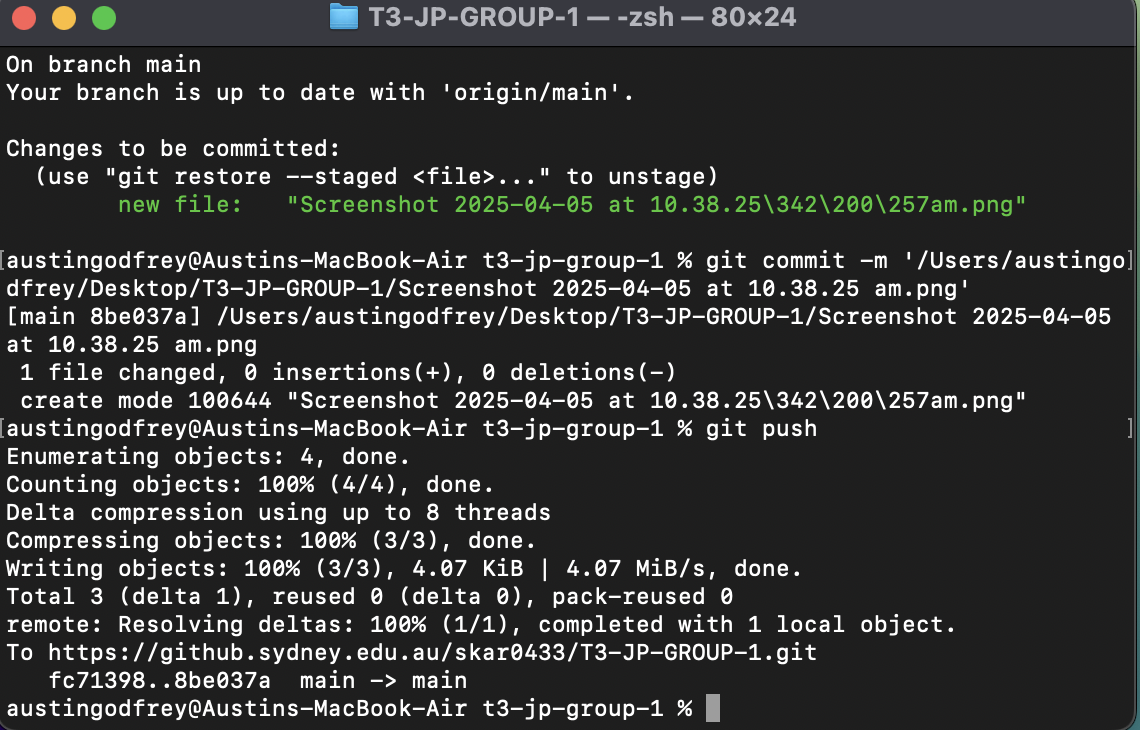
\includegraphics[width=0.8\textwidth]{austinpushfiles/push_to_main.png}}
 \newline
 
\textbf{Compiling latex file}
 \newline
 \centering{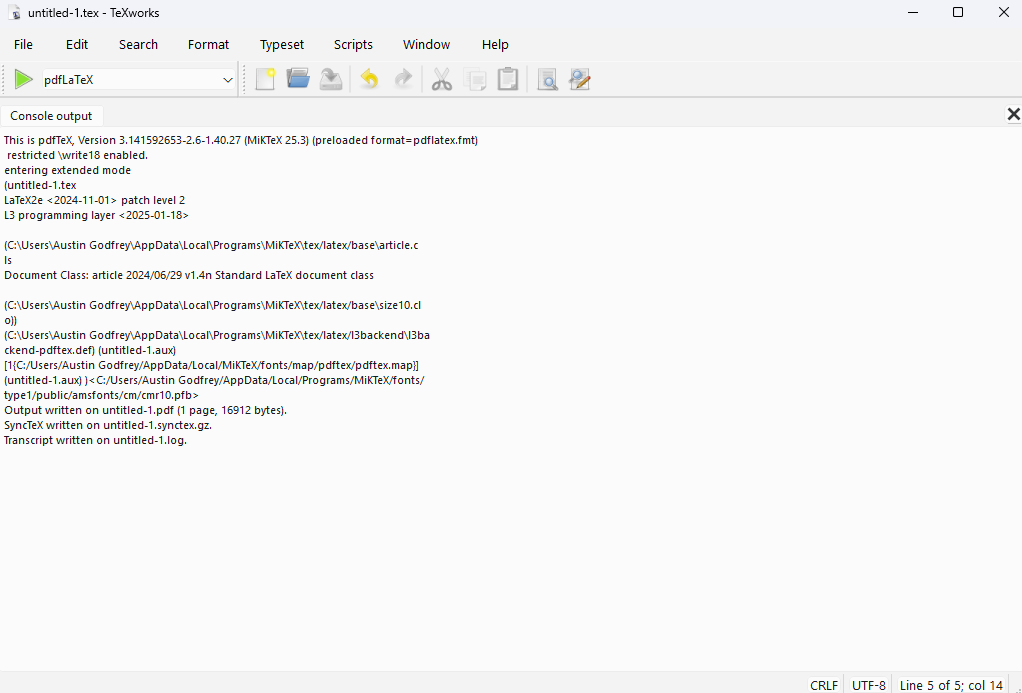
\includegraphics[width=0.8\textwidth]{austinpushfiles/compile_latex_file.png}}


\end{document}